This chapter lists the requirements for the effects presented in the analysis. 

\begin{figure}[htbp]
	\centering
\begin{picture}(0,0)%
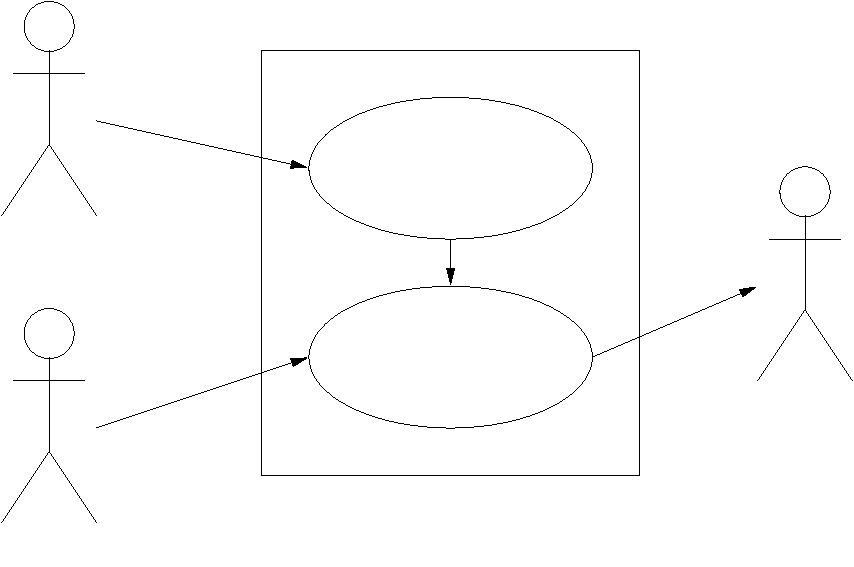
\includegraphics{Use_case.pdf}%
\end{picture}%
\setlength{\unitlength}{4144sp}%
%
\begingroup\makeatletter\ifx\SetFigFont\undefined%
\gdef\SetFigFont#1#2#3#4#5{%
  \reset@font\fontsize{#1}{#2pt}%
  \fontfamily{#3}\fontseries{#4}\fontshape{#5}%
  \selectfont}%
\fi\endgroup%
\begin{picture}(6507,4318)(1426,-4900)
\put(1531,-2491){User}%
\put(4546,-3346){Effect}%
\put(4276,-1906){Effect select}%
\put(7111,-3751){Amplifier}%
\put(1441,-4831){Guitar}%
\end{picture}%
	\caption{A graphically overview of wanted functionality in form of an use case digram.}
	\label{fig:use_case}
\end{figure}

The requirements are divided into units, based on the effect analysis \autoref{ch:analysing}, since it is concluded in \autoref{ch:analysing} that only six general units need to be designed and all the presented effects can be created with those six. The unit that are going to be designed are the:


\begin{itemize}
	\item Bandpass filter
	\item Inverse bandpass filter
	\item Delay
	\item Gain
	\item Clipping
	\item \gls{lfo}
\end{itemize} 

 Besides the fact that each unit shall be designed individually, each unit interface should fit in the effect that is using it. Each unit has its own section where the requirements and their arguments are presented. To ensure that the units can fit and work together, basic requirements  are made on the processing component to be chosen afterwards first.
 
 